\documentclass{article} % For LaTeX2e
\usepackage{graphicx}
\usepackage{caption}
\usepackage{subcaption}
\usepackage{amssymb}
\usepackage{amsmath}
\usepackage{nips14submit_e,times}
\usepackage{hyperref}
\usepackage{url}
%\usepackage{natbib}
%\documentstyle[nips14submit_09,times,art10]{article} % For LaTeX 2.09

\DeclareMathOperator{\x}{\mathbf{x}}
\DeclareMathOperator{\e}{\mathbf{e}}
\DeclareMathOperator{\M}{\mathbf{M}}
\DeclareMathOperator{\w}{\mathbf{w}}
\newcommand{\fix}{\marginpar{FIX}}
\newcommand{\new}{\marginpar{NEW}}
\edef\polishl{\l} 



\RequirePackage{latexsym}
\RequirePackage{amsmath}
\RequirePackage{amssymb} 
\RequirePackage{color} 
\RequirePackage{bm}
\RequirePackage{color}
\RequirePackage{picinpar}

%%%%%%%% Stock standard definitions %%%%%%%%%%%%%%%

\newcommand{\wbt}{\widetilde{\mathbf{w}}}
\DeclareMathOperator{\ab}{\mathbf{a}}
\DeclareMathOperator{\abh}{\widehat{\ab}}
\DeclareMathOperator{\bb}{\mathbf{b}}
\DeclareMathOperator{\bbh}{\widehat{\bb}}
\DeclareMathOperator{\cb}{\mathbf{c}}
\DeclareMathOperator{\db}{\mathbf{d}}
\DeclareMathOperator{\eb}{\mathbf{e}}
\DeclareMathOperator{\fb}{\mathbf{f}}
\DeclareMathOperator{\gb}{\mathbf{g}}
\DeclareMathOperator{\hb}{\mathbf{h}}
\DeclareMathOperator{\ib}{\mathbf{i}}
\DeclareMathOperator{\jb}{\mathbf{j}}
\DeclareMathOperator{\kb}{\mathbf{k}}
\DeclareMathOperator{\lb}{\mathbf{l}}
\DeclareMathOperator{\mb}{\mathbf{m}}
\DeclareMathOperator{\nbb}{\mathbf{n}}
\DeclareMathOperator{\ob}{\mathbf{o}}
\DeclareMathOperator{\pb}{\mathbf{p}}
\DeclareMathOperator{\qb}{\mathbf{q}}
\DeclareMathOperator{\rb}{\mathbf{r}}
\DeclareMathOperator{\sbb}{\mathbf{s}}
\DeclareMathOperator{\tb}{\mathbf{t}}
\DeclareMathOperator{\ub}{\mathbf{u}}
\DeclareMathOperator{\vb}{\mathbf{v}}
\DeclareMathOperator{\wb}{\mathbf{w}}
\DeclareMathOperator{\xb}{\mathbf{x}}
\DeclareMathOperator{\yb}{\mathbf{y}}
\DeclareMathOperator{\zb}{\mathbf{z}}
\renewcommand{\l}{\ell}

\DeclareMathOperator{\atilde}{\tilde{\ab}}
\DeclareMathOperator{\btilde}{\tilde{\bb}}
\DeclareMathOperator{\ctilde}{\tilde{\cb}}
\DeclareMathOperator{\dtilde}{\tilde{\db}}
\DeclareMathOperator{\etilde}{\tilde{\eb}}
\DeclareMathOperator{\ftilde}{\tilde{\fb}}
\DeclareMathOperator{\gtilde}{\tilde{\gb}}
\DeclareMathOperator{\htilde}{\tilde{\hb}}
\DeclareMathOperator{\itilde}{\tilde{\ib}}
\DeclareMathOperator{\jtilde}{\tilde{\jb}}
\DeclareMathOperator{\ktilde}{\tilde{\kb}}
\DeclareMathOperator{\ltilde}{\tilde{\lb}}
\DeclareMathOperator{\mtilde}{\tilde{\mb}}
\DeclareMathOperator{\ntilde}{\tilde{\nbb}}
\DeclareMathOperator{\otilde}{\tilde{\ob}}
\DeclareMathOperator{\ptilde}{\tilde{\pb}}
\DeclareMathOperator{\qtilde}{\tilde{\qb}}
\DeclareMathOperator{\rtilde}{\tilde{\rb}}
\DeclareMathOperator{\stilde}{\tilde{\sbb}}
\DeclareMathOperator{\ttilde}{\tilde{\tb}}
\DeclareMathOperator{\utilde}{\tilde{\ub}}
\DeclareMathOperator{\vtilde}{\tilde{\vb}}
\DeclareMathOperator{\wtilde}{\tilde{\wb}}
\DeclareMathOperator{\xtilde}{\tilde{\xb}}
\DeclareMathOperator{\ytilde}{\tilde{\yb}}
\DeclareMathOperator{\ztilde}{\tilde{\zb}}

\DeclareMathOperator{\abar}{\bar{\ab}}
\DeclareMathOperator{\bbar}{\bar{\bb}}
\DeclareMathOperator{\cbar}{\bar{\cb}}
\DeclareMathOperator{\dbar}{\bar{\db}}
\DeclareMathOperator{\ebar}{\bar{\eb}}
\DeclareMathOperator{\fbar}{\bar{\fb}}
\DeclareMathOperator{\gbar}{\bar{\gb}}
\DeclareMathOperator{\hbbar}{\bar{\hb}}
\DeclareMathOperator{\ibar}{\bar{\ib}}
\DeclareMathOperator{\jbar}{\bar{\jb}}
\DeclareMathOperator{\kbar}{\bar{\kb}}
\DeclareMathOperator{\lbar}{\bar{\lb}}
\DeclareMathOperator{\mbar}{\bar{\mb}}
\DeclareMathOperator{\nbar}{\bar{\nbb}}
\DeclareMathOperator{\obar}{\bar{\ob}}
\DeclareMathOperator{\pbar}{\bar{\pb}}
\DeclareMathOperator{\qbar}{\bar{\qb}}
\DeclareMathOperator{\rbar}{\bar{\rb}}
\DeclareMathOperator{\sbar}{\bar{\sbb}}
\DeclareMathOperator{\tbar}{\bar{\tb}}
\DeclareMathOperator{\ubar}{\bar{\ub}}
\DeclareMathOperator{\vbar}{\bar{\vb}}
\DeclareMathOperator{\wbar}{\bar{\wb}}
\DeclareMathOperator{\xbar}{\bar{\xb}}
\DeclareMathOperator{\ybar}{\bar{\yb}}
\DeclareMathOperator{\zbar}{\bar{\zb}}

\DeclareMathOperator{\Ab}{\mathbf{A}}
\DeclareMathOperator{\Bb}{\mathbf{B}}
\DeclareMathOperator{\Cb}{\mathbf{C}}
\DeclareMathOperator{\Db}{\mathbf{D}}
\DeclareMathOperator{\Eb}{\mathbf{E}}
\DeclareMathOperator{\Fb}{\mathbf{F}}
\DeclareMathOperator{\Gb}{\mathbf{G}}
\DeclareMathOperator{\Hb}{\mathbf{H}}
\DeclareMathOperator{\Ib}{\mathbf{I}}
\DeclareMathOperator{\Jb}{\mathbf{J}}
\DeclareMathOperator{\Kb}{\mathbf{K}}
\DeclareMathOperator{\Lb}{\mathbf{L}}
\DeclareMathOperator{\Mb}{\mathbf{M}}
\DeclareMathOperator{\Nb}{\mathbf{N}}
\DeclareMathOperator{\Ob}{\mathbf{O}}
\DeclareMathOperator{\Pb}{\mathbf{P}}
\DeclareMathOperator{\Qb}{\mathbf{Q}}
\DeclareMathOperator{\Rb}{\mathbf{R}}
\DeclareMathOperator{\Sbb}{\mathbf{S}}
\DeclareMathOperator{\Tb}{\mathbf{T}}
\DeclareMathOperator{\Ub}{\mathbf{U}}
\DeclareMathOperator{\Vb}{\mathbf{V}}
\DeclareMathOperator{\Wb}{\mathbf{W}}
\DeclareMathOperator{\Xb}{\mathbf{X}}
\DeclareMathOperator{\Xbt}{\widetilde{\Xb}}
\DeclareMathOperator{\Xbh}{\widehat{\Xb}}
\DeclareMathOperator{\Xbs}{\widetilde{\Xb}}
\DeclareMathOperator{\Zbs}{\widetilde{\Zb}}
\DeclareMathOperator{\Kbs}{\widetilde{\Kb}}
\DeclareMathOperator{\Zbh}{\widehat{\Zb}}
\DeclareMathOperator{\Ubh}{\widehat{\Ub}}
\DeclareMathOperator{\Yb}{\mathbf{Y}}
\DeclareMathOperator{\Zb}{\mathbf{Z}}

\DeclareMathOperator{\Abar}{\bar{A}}
\DeclareMathOperator{\Bbar}{\bar{B}}
\DeclareMathOperator{\Cbar}{\bar{C}}
\DeclareMathOperator{\Dbar}{\bar{D}}
\DeclareMathOperator{\Ebar}{\bar{E}}
\DeclareMathOperator{\Fbar}{\bar{F}}
\DeclareMathOperator{\Gbar}{\bar{G}}
\DeclareMathOperator{\Hbar}{\bar{H}}
\DeclareMathOperator{\Ibar}{\bar{I}}
\DeclareMathOperator{\Jbar}{\bar{J}}
\DeclareMathOperator{\Kbar}{\bar{K}}
\DeclareMathOperator{\Lbar}{\bar{L}}
\DeclareMathOperator{\Mbar}{\bar{M}}
\DeclareMathOperator{\Nbar}{\bar{N}}
\DeclareMathOperator{\Obar}{\bar{O}}
\DeclareMathOperator{\Pbar}{\bar{P}}
\DeclareMathOperator{\Qbar}{\bar{Q}}
\DeclareMathOperator{\Rbar}{\bar{R}}
\DeclareMathOperator{\Sbar}{\bar{S}}
\DeclareMathOperator{\Tbar}{\bar{T}}
\DeclareMathOperator{\Ubar}{\bar{U}}
\DeclareMathOperator{\Vbar}{\bar{V}}
\DeclareMathOperator{\Wbar}{\bar{W}}
\DeclareMathOperator{\Xbar}{\bar{X}}
\DeclareMathOperator{\Ybar}{\bar{Y}}
\DeclareMathOperator{\Zbar}{\bar{Z}}

\DeclareMathOperator{\Abbar}{\bar{\Ab}}
\DeclareMathOperator{\Bbbar}{\bar{\Bb}}
\DeclareMathOperator{\Cbbar}{\bar{\Cb}}
\DeclareMathOperator{\Dbbar}{\bar{\Db}}
\DeclareMathOperator{\Ebbar}{\bar{\Eb}}
\DeclareMathOperator{\Fbbar}{\bar{\Fb}}
\DeclareMathOperator{\Gbbar}{\bar{\Gb}}
\DeclareMathOperator{\Hbbar}{\bar{\Hb}}
\DeclareMathOperator{\Ibbar}{\bar{\Ib}}
\DeclareMathOperator{\Jbbar}{\bar{\Jb}}
\DeclareMathOperator{\Kbbar}{\bar{\Kb}}
\DeclareMathOperator{\Lbbar}{\bar{\Lb}}
\DeclareMathOperator{\Mbbar}{\bar{\Mb}}
\DeclareMathOperator{\Nbbar}{\bar{\Nb}}
\DeclareMathOperator{\Obbar}{\bar{\Ob}}
\DeclareMathOperator{\Pbbar}{\bar{\Pb}}
\DeclareMathOperator{\Qbbar}{\bar{\Qb}}
\DeclareMathOperator{\Rbbar}{\bar{\Rb}}
\DeclareMathOperator{\Sbbar}{\bar{\Sb}}
\DeclareMathOperator{\Tbbar}{\bar{\Tb}}
\DeclareMathOperator{\Ubbar}{\bar{\Ub}}
\DeclareMathOperator{\Vbbar}{\bar{\Vb}}
\DeclareMathOperator{\Wbbar}{\bar{\Wb}}
\DeclareMathOperator{\Xbbar}{\bar{\Xb}}
\DeclareMathOperator{\Ybbar}{\bar{\Yb}}
\DeclareMathOperator{\Zbbar}{\bar{\Zb}}

\DeclareMathOperator{\Ahat}{\widehat{A}}
\DeclareMathOperator{\Bhat}{\widehat{B}}
\DeclareMathOperator{\Chat}{\widehat{C}}
\DeclareMathOperator{\Dhat}{\widehat{D}}
\DeclareMathOperator{\Ehat}{\widehat{E}}
\DeclareMathOperator{\Fhat}{\widehat{F}}
\DeclareMathOperator{\Ghat}{\widehat{G}}
\DeclareMathOperator{\Hhat}{\widehat{H}}
\DeclareMathOperator{\Ihat}{\widehat{I}}
\DeclareMathOperator{\Jhat}{\widehat{J}}
\DeclareMathOperator{\Khat}{\widehat{K}}
\DeclareMathOperator{\Lhat}{\widehat{L}}
\DeclareMathOperator{\Mhat}{\widehat{M}}
\DeclareMathOperator{\Nhat}{\widehat{N}}
\DeclareMathOperator{\Ohat}{\widehat{O}}
\DeclareMathOperator{\Phat}{\widehat{P}}
\DeclareMathOperator{\Qhat}{\widehat{Q}}
\DeclareMathOperator{\Rhat}{\widehat{R}}
\DeclareMathOperator{\Shat}{\widehat{S}}
\DeclareMathOperator{\That}{\widehat{T}}
\DeclareMathOperator{\Uhat}{\widehat{U}}
\DeclareMathOperator{\Vhat}{\widehat{V}}
\DeclareMathOperator{\What}{\widehat{W}}
\DeclareMathOperator{\Xhat}{\widehat{X}}
\DeclareMathOperator{\Yhat}{\widehat{Y}}
\DeclareMathOperator{\Zhat}{\widehat{Z}}

\DeclareMathOperator{\Abhat}{\widehat{\Ab}}
\DeclareMathOperator{\Bbhat}{\widehat{\Bb}}
\DeclareMathOperator{\Cbhat}{\widehat{\Cb}}
\DeclareMathOperator{\Dbhat}{\widehat{\Db}}
\DeclareMathOperator{\Ebhat}{\widehat{\Eb}}
\DeclareMathOperator{\Fbhat}{\widehat{\Fb}}
\DeclareMathOperator{\Gbhat}{\widehat{\Gb}}
\DeclareMathOperator{\Hbhat}{\widehat{\Hb}}
\DeclareMathOperator{\Ibhat}{\widehat{\Ib}}
\DeclareMathOperator{\Jbhat}{\widehat{\Jb}}
\DeclareMathOperator{\Kbhat}{\widehat{\Kb}}
\DeclareMathOperator{\Lbhat}{\widehat{\Lb}}
\DeclareMathOperator{\Mbhat}{\widehat{\Mb}}
\DeclareMathOperator{\Nbhat}{\widehat{\Nb}}
\DeclareMathOperator{\Obhat}{\widehat{\Ob}}
\DeclareMathOperator{\Pbhat}{\widehat{\Pb}}
\DeclareMathOperator{\Qbhat}{\widehat{\Qb}}
\DeclareMathOperator{\Rbhat}{\widehat{\Rb}}
\DeclareMathOperator{\Sbhat}{\widehat{\Sb}}
\DeclareMathOperator{\Tbhat}{\widehat{\Tb}}
\DeclareMathOperator{\Ubhat}{\widehat{\Ub}}
\DeclareMathOperator{\Vbhat}{\widehat{\Vb}}
\DeclareMathOperator{\Wbhat}{\widehat{\Wb}}
\DeclareMathOperator{\Xbhat}{\widehat{\Xb}}
\DeclareMathOperator{\Ybhat}{\widehat{\Yb}}
\DeclareMathOperator{\Zbhat}{\widehat{\Zb}}

\DeclareMathOperator{\Acal}{\mathcal{A}}
\DeclareMathOperator{\Bcal}{\mathcal{B}}
\DeclareMathOperator{\Ccal}{\mathcal{C}}
\DeclareMathOperator{\Dcal}{\mathcal{D}}
\DeclareMathOperator{\Ecal}{\mathcal{E}}
\DeclareMathOperator{\Fcal}{\mathcal{F}}
\DeclareMathOperator{\Gcal}{\mathcal{G}}
\DeclareMathOperator{\Hcal}{\mathcal{H}}
\DeclareMathOperator{\Ical}{\mathcal{I}}
\DeclareMathOperator{\Jcal}{\mathcal{J}}
\DeclareMathOperator{\Kcal}{\mathcal{K}}
\DeclareMathOperator{\Lcal}{\mathcal{L}}
\DeclareMathOperator{\Mcal}{\mathcal{M}}
\DeclareMathOperator{\Ncal}{\mathcal{N}}
\DeclareMathOperator{\Ocal}{\mathcal{O}}
\DeclareMathOperator{\Pcal}{\mathcal{P}}
\DeclareMathOperator{\Qcal}{\mathcal{Q}}
\DeclareMathOperator{\Rcal}{\mathcal{R}}
\DeclareMathOperator{\Scal}{\mathcal{S}}
\DeclareMathOperator{\Scalt}{\widetilde{\Scal}}
\DeclareMathOperator{\Tcal}{\mathcal{T}}
\DeclareMathOperator{\Ucal}{\mathcal{U}}
\DeclareMathOperator{\Vcal}{\mathcal{V}}
\DeclareMathOperator{\Wcal}{\mathcal{W}}
\DeclareMathOperator{\Xcal}{\mathcal{X}}
\DeclareMathOperator{\Ycal}{\mathcal{Y}}
\DeclareMathOperator{\Zcal}{\mathcal{Z}}

\DeclareMathOperator{\Atilde}{\widetilde{A}}
\DeclareMathOperator{\Btilde}{\widetilde{B}}
\DeclareMathOperator{\Ctilde}{\widetilde{C}}
\DeclareMathOperator{\Dtilde}{\widetilde{D}}
\DeclareMathOperator{\Etilde}{\widetilde{E}}
\DeclareMathOperator{\Ftilde}{\widetilde{F}}
\DeclareMathOperator{\Gtilde}{\widetilde{G}}
\DeclareMathOperator{\Htilde}{\widetilde{H}}
\DeclareMathOperator{\Itilde}{\widetilde{I}}
\DeclareMathOperator{\Jtilde}{\widetilde{J}}
\DeclareMathOperator{\Ktilde}{\widetilde{K}}
\DeclareMathOperator{\Ltilde}{\widetilde{L}}
\DeclareMathOperator{\Mtilde}{\widetilde{M}}
\DeclareMathOperator{\Ntilde}{\widetilde{N}}
\DeclareMathOperator{\Otilde}{\widetilde{O}}
\DeclareMathOperator{\Ptilde}{\widetilde{P}}
\DeclareMathOperator{\Qtilde}{\widetilde{Q}}
\DeclareMathOperator{\Rtilde}{\widetilde{R}}
\DeclareMathOperator{\Stilde}{\widetilde{S}}
\DeclareMathOperator{\Ttilde}{\widetilde{T}}
\DeclareMathOperator{\Utilde}{\widetilde{U}}
\DeclareMathOperator{\Vtilde}{\widetilde{V}}
\DeclareMathOperator{\Wtilde}{\widetilde{W}}
\DeclareMathOperator{\Xtilde}{\widetilde{X}}
\DeclareMathOperator{\Ytilde}{\widetilde{Y}}
\DeclareMathOperator{\Ztilde}{\widetilde{Z}}


%%%%%%%% Widely accepted definitions %%%%%%%%%%%%%%%

\DeclareMathOperator{\CC}{\mathbb{C}} % Complex numbers
\DeclareMathOperator{\EE}{\mathbb{E}} % Expectation
\DeclareMathOperator{\KK}{\mathbb{K}} % Arbitrary field
\DeclareMathOperator{\MM}{\mathbb{M}} % Median
\DeclareMathOperator{\NN}{\mathbb{N}} % Natural numbers
\DeclareMathOperator{\PP}{\mathbb{P}} % Probability
\DeclareMathOperator{\QQ}{\mathbb{Q}} % Rationals
\DeclareMathOperator{\RR}{\mathbb{R}} % Real numbers 
\DeclareMathOperator{\ZZ}{\mathbb{Z}} % Integers

\DeclareMathOperator{\one}{\mathbf{1}}  % Identity
\DeclareMathOperator{\zero}{\mathbf{0}} % Zero
\DeclareMathOperator{\TRUE}{\mathbf{TRUE}}  % True
\DeclareMathOperator{\FALSE}{\mathbf{FALSE}}  % False

\DeclareMathOperator*{\mini}{\mathop{\mathrm{minimize}}}
\DeclareMathOperator*{\maxi}{\mathop{\mathrm{maximize}}}
\DeclareMathOperator*{\argmin}{\mathop{\mathrm{argmin}}}
\DeclareMathOperator*{\argmax}{\mathop{\mathrm{argmax}}}
\DeclareMathOperator*{\argsup}{\mathop{\mathrm{argsup}}}
\DeclareMathOperator*{\arginf}{\mathop{\mathrm{arginf}}}
\DeclareMathOperator{\sgn}{\mathop{\mathrm{sign}}}
\DeclareMathOperator{\sign}{\mathop{\mathrm{sign}}}
\DeclareMathOperator{\tr}{\mathop{\mathrm{tr}}}
\DeclareMathOperator{\rank}{\mathop{\mathrm{rank}}}
\DeclareMathOperator{\traj}{\mathop{\mathrm{Traj}}}

%%%%%%%% Bold Greek Letters %%%%%%%%%%%%%%%
\DeclareMathOperator{\sigmab}{\bm{\sigma}}
\DeclareMathOperator{\Sigmab}{\mathbf{\Sigma}}


%%%%%%%% Mess around with LaTeX %%%%%%%%%%%%%%%

%% Some style files might actually define these variables.
%% So don't mess with them if they are already defined

\ifx\BlackBox\undefined
\newcommand{\BlackBox}{\rule{1.5ex}{1.5ex}}  % end of proof
\fi

\ifx\proof\undefined
\newenvironment{proof}{\par\noindent{\bf Proof\ }}{\hfill\BlackBox\\[2mm]}
% \else
% \renewenvironment{proof}{\par\noindent{\bf Proof\ }}{\hfill\BlackBox\\[2mm]}
\fi

%Trying to put all on Section track
%\makeatletter
%\@addtoreset{equation}{section}
%\def\theequation{\thesection.\arabic{equation}}
%\def\thetheorem{\thesection.\arabic{theorem}}
%\makeatother

%the below clashes with the previous defs of them... 
%in the style files
%\newtheorem{theorem}{Theorem}[section]
%\newtheorem{lemma}[theorem]{Lemma}
%\newtheorem{corollary}[theorem]{Corollary}
%\newtheorem{conjecture}[conjecture]{Conjecture}


%%%%%%%% Utility functions %%%%%%%%%%%%%%%

\newcommand{\eq}[1]{(\ref{#1})} 
\newcommand{\mymatrix}[2]{\left[\begin{array}{#1} #2 \end{array}\right]}
\newcommand{\mychoose}[2]{\left(\begin{array}{c} #1 \\ #2 \end{array}\right)}
\newcommand{\mydet}[1]{\det\left[ #1 \right]}
\newcommand{\sembrack}[1]{[\![#1]\!]}

\newcommand{\ea}{\emph{et al. }}
\newcommand{\eg}{\emph{e.g. }}
\newcommand{\ie}{\emph{i.e., }}

\newcommand{\mnote}[1]{\marginpar{#1}}
\newcommand{\note}[1]{{\bf {#1}}}

%%%%%%%% Specific symbols for this project %%%%%%%%%%%%%%%

\DeclareMathOperator{\half}{\frac{1}{2}}

\newcommand{\Ref}[1]{\hfill\Green{[#1]}}
\DeclareMathOperator{\XX}{\mathcal{X}}
\newcommand{\ar}{\implies}
\newcommand{\yh}{\hat{y}}
\DeclareMathOperator{\lan}{\langle}
\DeclareMathOperator{\ran}{\rangle}

\DeclareMathOperator{\dc}{\mathrm{dc}}

\DeclareMathOperator{\Utb}{\widetilde{\Ub}}
\DeclareMathOperator{\Stb}{\widetilde{\Sbb}}

\ifx\Brown\undefined
\definecolor{brown}{rgb}{0.5,0.1,0.1}
\newcommand{\Brown}[1]{\color{brown}{#1}\color{black}}
\fi

\ifx\Red\undefined
\definecolor{red}{rgb}{1.0,0,0}
\newcommand{\Red}[1]{\color{red}{#1}\color{black}}
\fi

\ifx\Green\undefined
\definecolor{green}{rgb}{0,0.4,0}
\newcommand{\Green}[1]{\color{green}{#1}\color{black}}
\fi

\ifx\Blue\undefined
\definecolor{blue}{rgb}{0,0,1.0}
\newcommand{\Blue}[1]{\color{blue}{#1}\color{black}}
\fi



\newcommand{\beq}{\begin{equation}}
\newcommand{\eeq}{\end{equation}}
\newcommand{\beh}{\begin{conjecture}}
\newcommand{\eeh}{\end{conjecture}}
\newcommand\bel{\begin{lemma}}
\newcommand\eel{\end{lemma}}
\newcommand\bet{\begin{theoreme}}
\newcommand\eet{\end{theoreme}}
\newcommand\bex{\begin{example}}
\newcommand\eex{\end{example}}
\newcommand\bed{\begin{definition}}
\newcommand\eed{\end{definition}}
\newcommand\bep{\begin{proposition}}
\newcommand\eep{\end{proposition}}
\newcommand\ber{\begin{remark}}
\newcommand\eer{\end{remark}}
\newcommand\bec{\begin{corollary}}
\newcommand\eec{\end{corollary}}
%\newcommand\proof{\noindent {\bf Proof.}\ \ }
\newcommand\qed{\hfill$\Box$\medskip}
\newcommand\cP{{\mathcal P}}
\newcommand\cJ{{\mathcal J}}
\newcommand\cD{{\mathcal D}}
\newcommand\cC{{\mathcal C}}
\newcommand\cO{{\mathcal O}}
\newcommand\cS{{\mathcal S}}
\newcommand\cT{{\mathcal T}}
\newcommand\cV{{\mathcal V}}
\newcommand\cW{{\mathcal W}}
\newcommand\cY{{\mathcal Y}}
\newcommand\cF{{\mathcal F}}
\newcommand\cU{{\mathcal U}}
\newcommand\cE{{\mathcal E}}
\newcommand\cG{{\mathcal G}}
\newcommand\cB{{\mathcal B}}
\newcommand\cI{{\rm I}}
\newcommand\cN{{\mathcal N}}
\newcommand\cM{{\mathcal M}}
\newcommand\cA{{\mathcal A}}
\newcommand\cQ{{\mathcal Q}}
\newcommand\cK{{\mathcal K}}
\newcommand\cZ{{\mathcal Z}}
\newcommand\CAP{{\rm cap}}
\newcommand\ENT{{\rm ent}}
\newcommand\gr{{\rm gr}}

\def\qq{{\mathbb Q}}
\def\ff{{\mathbb F}}
\def\rr{{\mathbb R}}
\def\zz{{\mathbb Z}}
\def\cc{{\mathbb C}}
\def\nn{{\mathbb N}}
\def\kk{{\mathbb K}}
\def\ee{{\mathbb E}}
\def\ww{{\mathbb W}}
\def\hh{{\mathbb H}}
\def\ss{{\mathbb S}}
\def\tt{{\mathbb T}}
\def\pp{{\mathbb P}}



\newtheorem{theoreme}{Theorem} %[section]
\newtheorem{proposition}[theoreme]{Proposition}
\newtheorem{lemma}[theoreme]{Lemma}
\newtheorem{definition}[theoreme]{Definition}
\newtheorem{corollary}[theoreme]{Corollary}
\newtheorem{remark}[theoreme]{Remark}
\newtheorem{example}[theoreme]{Example}
\newtheorem{examples}[theoreme]{Examples}
%\newtheorem{conjecture}[theoreme]{Conjecture}
\newtheorem{conjecture}{Conjecture}


\title{An Information Theoretic Approach to Measuring Text Interestingness}


\author{
David S.~Hippocampus\thanks{ Use footnote for providing further information
about author (webpage, alternative address)---\emph{not} for acknowledging
funding agencies.} \\
Department of Computer Science\\
Cranberry-Lemon University\\
Pittsburgh, PA 15213 \\
\texttt{hippo@cs.cranberry-lemon.edu} \\
\And
Coauthor \\
Affiliation \\
Address \\
\texttt{email} \\
\AND
Coauthor \\
Affiliation \\
Address \\
\texttt{email} \\
\And
Coauthor \\
Affiliation \\
Address \\
\texttt{email} \\
\And
Coauthor \\
Affiliation \\
Address \\
\texttt{email} \\
(if needed)\\
}

% The \author macro works with any number of authors. There are two commands
% used to separate the names and addresses of multiple authors: \And and \AND.
%
% Using \And between authors leaves it to \LaTeX{} to determine where to break
% the lines. Using \AND forces a linebreak at that point. So, if \LaTeX{}
% puts 3 of 4 authors names on the first line, and the last on the second
% line, try using \AND instead of \And before the third author name.

%\newcommand{\fix}{\marginpar{FIX}}
%\newcommand{\new}{\marginpar{NEW}}

%\nipsfinalcopy % Uncomment for camera-ready version

\begin{document}


\maketitle

\begin{abstract}

We investigate the problem of automatic prediction of text interestingness and present an information theoretic approach for quantifying text interestingness in terms of text topic diversity.  Our hypothesis is, in many text domains, often an interesting concept is generated by mixing a diverse set of topics.  Given a word distributional model learned from text corpus, we present an algorithm that leverages {\sl Jensen-Shannon} divergence for measuring text diversity and demonstrate how such a measure correlates with text interestingness. We describe several different base-line algorithms and present results over two different data sets: a collection of e-commerce products from {\sl eBay} , and a collection of  {\sl NSF} Awards from $2007$ to $2012$. 
\end{abstract}


%%%%%%%%%%%%%%%%%%%%%%%%%%%%%%%%%%%%%%%%%%%%%%%%%%%%%%%%%%%%%
%%%%%%%%%%%%%%%%%%%%%%%%%%%%%%%%%%%%%%%%%%%%%%%%%%%%%%%%%%%%%
%%%%%%%%%%%%%%%%%%%%%%%%%%%%%%%%%%%%%%%%%%%%%%%%%%%%%%%%%%%%%

\section{Introduction}
\label{sec:introduction}

\begin{figure}
        \centering
        \begin{subfigure}[b]{0.3\textwidth}
                \centering
                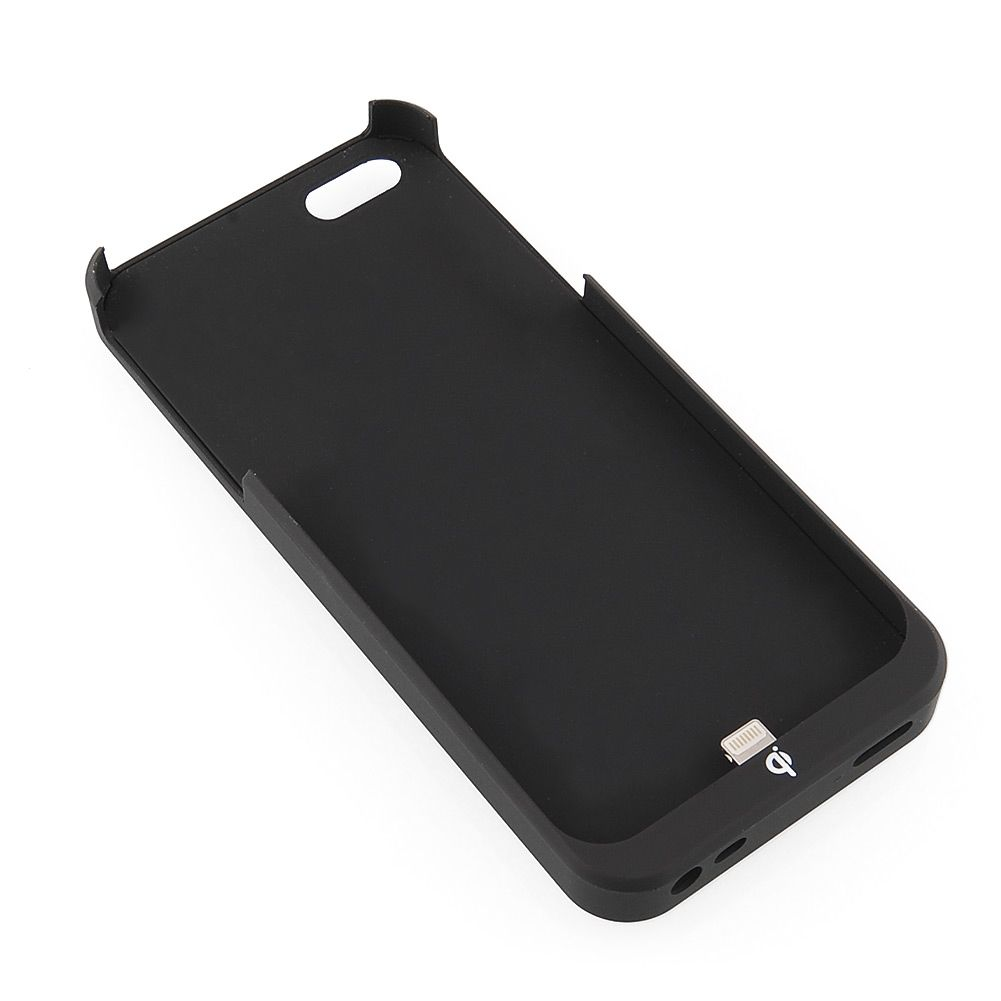
\includegraphics[width=\textwidth]{figures/standard-iphone-case.jpg}
                \caption{Black Qi Standard Wireless Charging Charger Receiver Case For iPhone 5 5G}
                \label{fig:standard-iphone-case}
        \end{subfigure}%
              ~ %add desired spacing between images, e. g. ~, \quad, \qquad, \hfill etc.
          %(or a blank line to force the subfigure onto a new line)
        \begin{subfigure}[b]{0.3\textwidth}
                \centering
                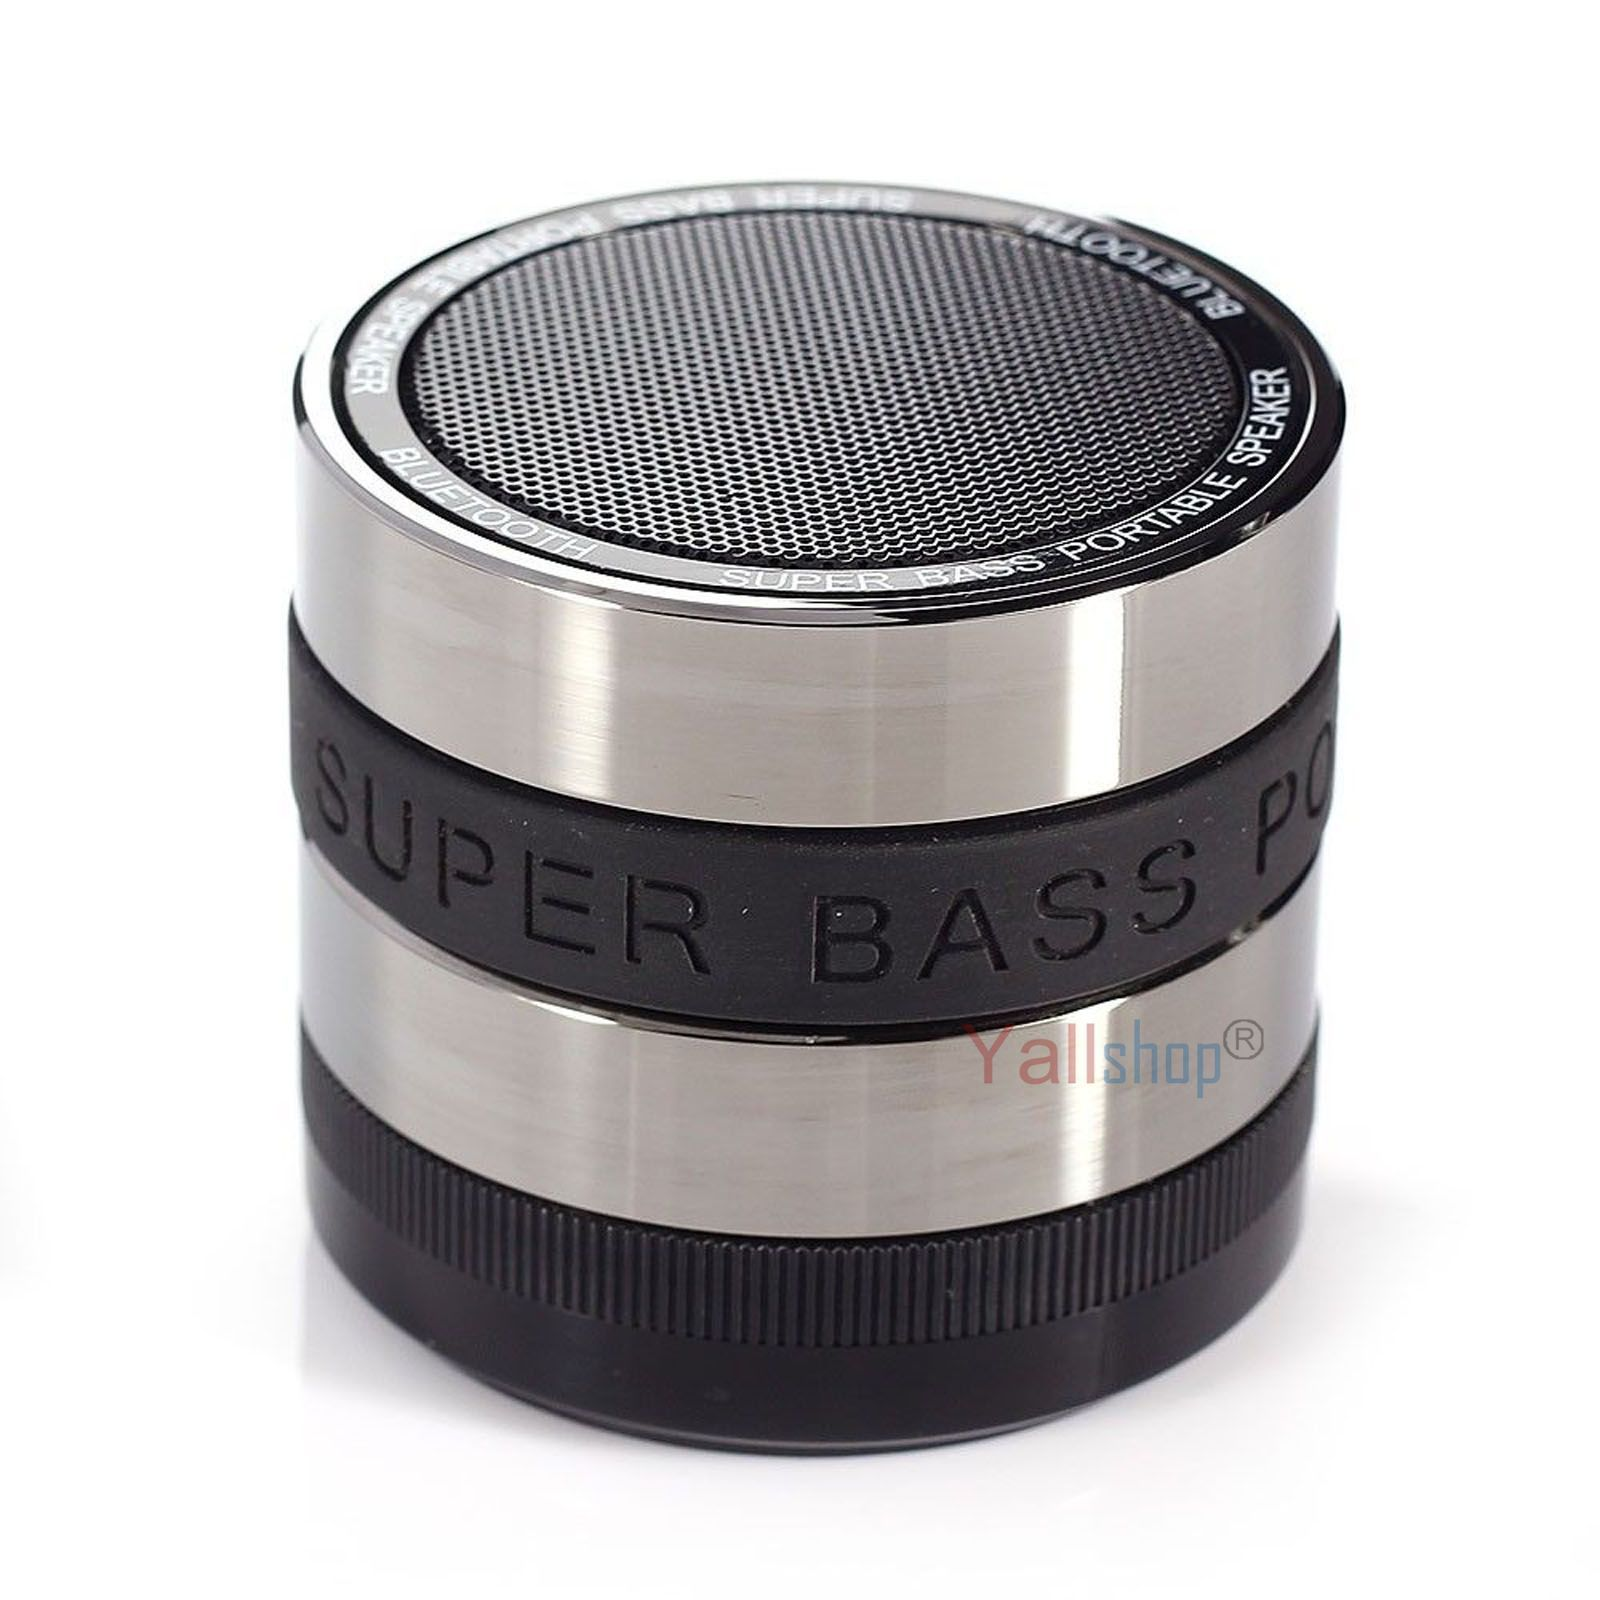
\includegraphics[width=\textwidth]{figures/standard-iphone-speaker.jpg}
                \caption{Bluetooth Wireless Speaker Mini Portable Super Bass For iPhone}
                \label{fig:standard-speaker}
        \end{subfigure}%
              ~ %add desired spacing between images, e. g. ~, \quad, \qquad, \hfill etc.
          %(or a blank line to force the subfigure onto a new line)
        \begin{subfigure}[b]{0.3\textwidth}
                \centering
                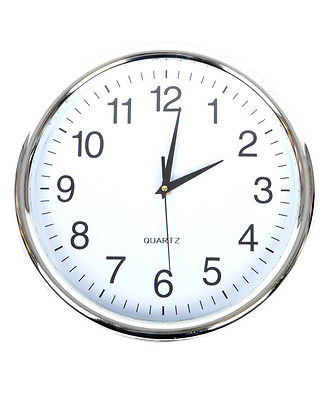
\includegraphics[width=\textwidth]{figures/standard-clock.jpg}
                \caption{The Standard Round Wall Clock (C9207)}
                \label{fig:standard-speaker}
        \end{subfigure}\\
        ~ %add desired spacing between images, e. g. ~, \quad, \qquad, \hfill etc.
          %(or a blank line to force the subfigure onto a new line)
        \begin{subfigure}[b]{0.3\textwidth}
        	        \centering
                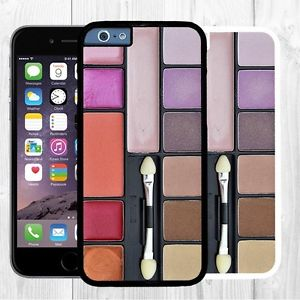
\includegraphics[width=\textwidth]{figures/eyeshadow-iphone-case.jpg}
                \caption{\textcolor{red}{{\bf Eyeshadow}} Palettes for \textcolor{red}{{\bf iPhone}} 6 case}
                \label{fig:eyeshadow-iphone-case}
        \end{subfigure}
              ~ %add desired spacing between images, e. g. ~, \quad, \qquad, \hfill etc.
          %(or a blank line to force the subfigure onto a new line)
        \begin{subfigure}[b]{0.3\textwidth}
                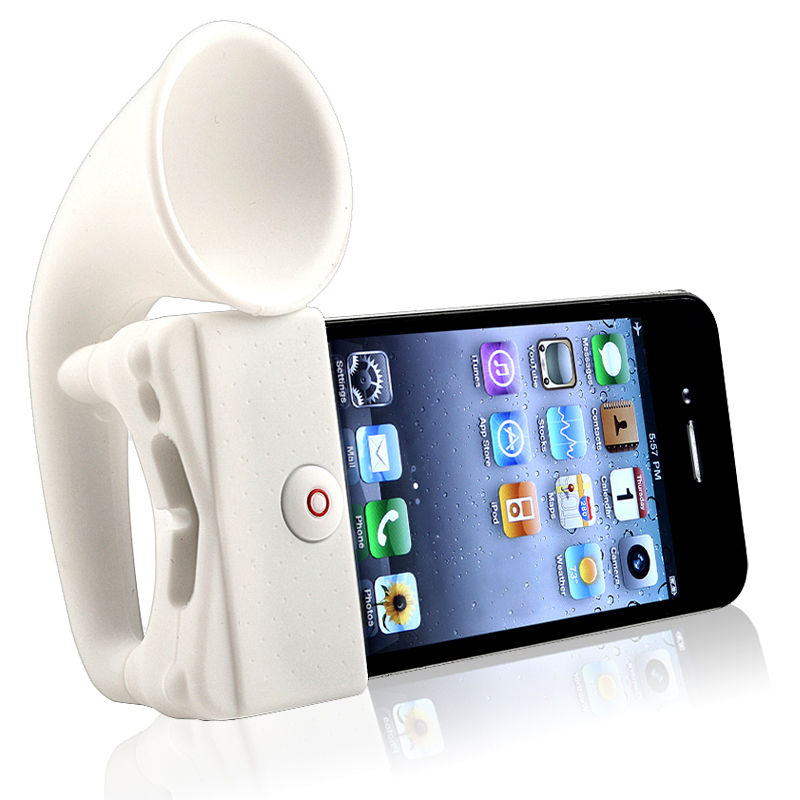
\includegraphics[width=\textwidth]{figures/horn-iphone-speaker.jpg}
                \caption{White Silicone \textcolor{red}{{\bf Horn}} Stand Speaker for Apple \textcolor{red}{{\bf iPhone}} 4/ 4S}
                \label{fig:zeppelin-speaker}
        \end{subfigure}
       ~ %add desired spacing between images, e. g. ~, \quad, \qquad, \hfill etc.
          %(or a blank line to force the subfigure onto a new line)
        \begin{subfigure}[b]{0.35\textwidth}
                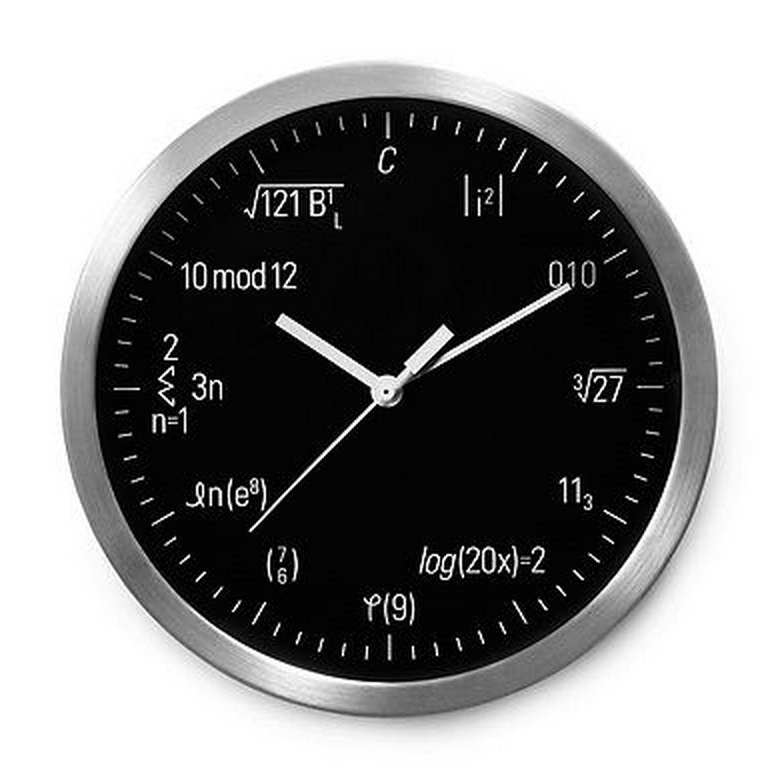
\includegraphics[width=\textwidth]{figures/geeky-clock}
                \caption{\textcolor{red}{{\bf Equation}} Wall \textcolor{red}{{\bf Clock}} Gifts for Math Gurus or Best Geek Friends}
                \label{fig:geeky-clock}
        \end{subfigure}
       \caption{Pictures of animals}\label{fig:animals}
\end{figure}

%%%%%%%%%%%%%%%%%%%%%%%%%%%%%%%%%%%%%%%%%%%%%%%%%%%%%%%%%%%%%
%%%%%%%%%%%%%%%%%%%%%%%%%%%%%%%%%%%%%%%%%%%%%%%%%%%%%%%%%%%%%
%%%%%%%%%%%%%%%%%%%%%%%%%%%%%%%%%%%%%%%%%%%%%%%%%%%%%%%%%%%%%

\section{Our Approach}
\label{sec:our-approach}
As a starting point of our model, we assume that we can describe any
word with a probability distribution over a fixed set of topics -
e.g. learned from a topic model. Now, given a small
set of words, we in effect have a set of topic distributions. Let us
denote the set of words by $S=\{w_1,...,w_k\}$, and the distribution
of a word $w$ by $P_w$.  We now ask
what is the diversity of the set of probability
distributions $\cP_S=\{P_{w_1},...,P_{w_k}\}$? To make this task
somewhat more concrete, we make some 
assumptions of what we expect from the measure. First, if the set
$\cP_S$ only contains one element, then it is not diverse. Moreover,
we have a certain fixed {\em prior} distribution $P$, which we
can think of as the overall distribution of topics. If a distribution
$P_{w_i}$ is equal to $P$, then it does not carry any information, so
it should not have any impact on the diversity of $\cP_S$. In
accordance with those assumptions, we will will introduce some basic
notation. Let $D_{KL}(\centerdot\|\centerdot)$ denote the
Kullback-Leibler Divergence.

\bed
Given a distribution $P_w$, its {\bf importance} with respect to a
prior distribution $P$ is defined as 
\[D_w = D_{KL}(P_w\|P).\]
\eed

\bed\label{mixture}
Given a set of distributions $\cP_S=\{P_{w_1},...,P_{w_k}\}$ and a
prior $P$, we
define a mixture distribution $P_S$ as
\[P_S=\sum_{i=1}^k d_{w_i} P_{w_i},\]
where $d_{w_i}=\frac{D_{w_i}}{\sum D_{w_j}}$ are the normalized
importances.
\eed

Essentially, $P_S$ is the weighted average of the set $\cP_S$, where
the weights are chosen according to the importances. Now, we can
define the diversity measure.

\bed\label{diversity}
We define the Jensen-Shannon Information Diversity of a set of
distributions $\cP_S$ with respect to 
prior $P$ as
\[D_S=\sum_{i=1}^k d_{w_i}D_{KL}(P_{w_i}\|P_S), \]
where $d_{w_i}$ and $P_S$ are as in the previous definition.
\eed
This definition is closely related to the 
{\em general Jensen-Shannon Divergence}, defined in [topsoe]. Another
interesting theoretical property of Jensen-Shannon Information
Diversity is that it can be interpreted as a generalization of Shannon
entropy as a population diversity measure, however we will not go
into this here any further. 

 Applying this general model to the natural language requires some
 additional considerations. First, how do we obtain a topic
 ditribution for a given word, and what is the prior topic
 distribution. As the terminology suggests, we want to rely on a topic
 model. Specifically, suppose we have a set $T$ of documents, sentences or
 paragraphs of any length, in which we want to find the most diverse
 examples. Additionally, we have a large set $D$ of documents which
 has content {\em similar} to $T$. We will train a topic model on $D$,
 and use it analyzing $T$. Of course, both sets could be identical,
 but $T$ may, for example, be a set of sentences or short messages,
which not suitable for training a good topic model on. In those cases,
as we will see, the fact that $T$ and $D$ do not 
 need to be identical will give our method a distinct advantage over
 competing approaches. The key component we will need from the topic
 model is the word-topic matrix $M$, where $M_{ij}$ is the number of
 times $i$-th word was assigned the $j$-th topics. So, if we
 probabilistically normalize
 the $i$-th row of $M$, it will be the topic assignment distribution
 for the $i$-th word in our dictionary. This is a good candidate for a
 topic distribution to use in our model. Similarly, we obtain a prior
 topic distribution by computing the proportions of overall topic
 assignments. This corresponds to summing up matrix $M$ along its
 columns, and then normalizing the resulting vector.

The proposed choice of topic distributions for words has some
shortcomings. First, consider a word $w$ which occurs only once (or very
few times in the entire set $D$. Then, its topic distribution will be
very concentrated. Assuming that the prior distribution is close to
uniform, that will give a very high importance to $w$, just because
there is not enough datapoints in our set to determine its {\em true}
topic distribution. 

Furthermore, if we interpret a topic distribution as representing the
{\em meaning} of a word, then having a fixed distribution for each
word would not be able to reflect the fact that words often have
different meanings in different contexts. In effect, all of the
meanings would be combined together, and likely the most frequent one
would dominate, distorting the results.







%%%%%%%%%%%%%%%%%%%%%%%%%%%%%%%%%%%%%%%%%%%%%%%%%%%%%%%%%%%%%
%%%%%%%%%%%%%%%%%%%%%%%%%%%%%%%%%%%%%%%%%%%%%%%%%%%%%%%%%%%%%
%%%%%%%%%%%%%%%%%%%%%%%%%%%%%%%%%%%%%%%%%%%%%%%%%%%%%%%%%%%%%

\section{Experiments}
\label{sec:experiments}

\subsection{Data Sets}
\label{sec:data-sets}
\begin{itemize}
\item {\bf iPhone cases:}
\item{\bf NSF:}
\end{itemize}

\subsection{Baselines}
\label{sec:baselines}

Diversity:
\begin{itemize}
\item {\bf Shannon  Entropy:}
\item{\bf Topic Diversity:} \cite{ganguly:2014}, \cite{bache:2013}
\item{\bf Word frequency as distribution:}
\end{itemize}



Classification:
\begin{itemize}
\item {\bf Bag of words (BOW):}
\item{\bf Latent Semantic Indexing (LSI):}
\item{\bf Recursive Auto Encoders (RAE):}
\end{itemize}

\subsection{Results}
\label{sec:results}


%%%%%%%%%%%%%%%%%%%%%%%%%%%%%%%%%%%%%%%%%%%%%%%%%%%%%%%%%%%%%
%%%%%%%%%%%%%%%%%%%%%%%%%%%%%%%%%%%%%%%%%%%%%%%%%%%%%%%%%%%%%
%%%%%%%%%%%%%%%%%%%%%%%%%%%%%%%%%%%%%%%%%%%%%%%%%%%%%%%%%%%%%

\section{Conclusions}
\label{sec:conclusions}

%%%%%%%%%%%%%%%%%%%%%%%%%%%%%%%%%%%%%%%%%%%%%%%%%%%%%%%%%%%%%
%%%%%%%%%%%%%%%%%%%%%%%%%%%%%%%%%%%%%%%%%%%%%%%%%%%%%%%%%%%%%
%%%%%%%%%%%%%%%%%%%%%%%%%%%%%%%%%%%%%%%%%%%%%%%%%%%%%%%%%%%%%

\begin{figure}[h]
\begin{center}
%\framebox[4.0in]{$\;$}
\fbox{\rule[-.5cm]{0cm}{4cm} \rule[-.5cm]{4cm}{0cm}}
\end{center}
\caption{Sample figure caption.}
\end{figure}



\begin{table}[t]
\caption{Sample table title}
\label{sample-table}
\begin{center}
\begin{tabular}{ll}
\multicolumn{1}{c}{\bf PART}  &\multicolumn{1}{c}{\bf DESCRIPTION}
\\ \hline \\
Dendrite         &Input terminal \\
Axon             &Output terminal \\
Soma             &Cell body (contains cell nucleus) \\
\end{tabular}
\end{center}
\end{table}

%%%%%%%%%%%%%%%%%%%%%%%%%%%%%%%%%%%%%%%%%%%%%%%%%%%%%%%%%%%%%
%%%%%%%%%%%%%%%%%%%%%%%%%%%%%%%%%%%%%%%%%%%%%%%%%%%%%%%%%%%%%
%%%%%%%%%%%%%%%%%%%%%%%%%%%%%%%%%%%%%%%%%%%%%%%%%%%%%%%%%%%%%

\bibliographystyle{plain}
\bibliography{nips2014}


\end{document}
